\documentclass{beamer}

\usepackage{listings}
\usepackage[T1]{fontenc}
\usepackage{multicol}
\usepackage{graphicx}
\usepackage{courier}
\usepackage{ragged2e}

\title{GameL}
\subtitle{The Game Scripting Language}
\author{Tianyu Cheng\\ Ben Lin\\ Mark Mansi}

\usetheme{Boadilla}
\usecolortheme{beetle}

\lstset{basicstyle=\footnotesize\ttfamily, breaklines=true}

\begin{document}

% title frame
\begin{frame}
    \maketitle
\end{frame}

\begin{frame}
    \frametitle{What is GameL?}
    \begin{columns}[T]
    \begin{column}[T]{5cm}
    \begin{itemize}[<+->]
        \item{A scripting language}
        \item{Designed to abstract game constructs}
        \item{Flexible}
        \item{Integrated with Java/Scala Swing}
    \end{itemize}
    \end{column}
    \begin{column}[T]{5cm}
        
\includegraphics[width=5cm]{../res/icon}
    \end{column}
    \end{columns}
\end{frame}

\begin{frame}
    \frametitle{What is GameL?}
    \begin{columns}[T]
    \begin{column}[T]{5cm}
    Abstrations:
    \begin{itemize}
        \item<1-> Entities
        \item<2-> Ownership
        \item<3-> Actions
        \item<4-> Scenes
        \item<5-> Transitions
    \end{itemize}
    \end{column}
    \begin{column}[T]{5cm}
        \includegraphics<1>[width=7cm]{foo}
        \visible<2>{
            \includegraphics<2>[width=5cm]{ownership}

            \tiny{http://forums.ubi.com/archive/index.php/t-775003.html}
        }
        \visible<3>{
            \includegraphics<3>[width=5cm]{action}

           \tiny{http://properpropaganda.net/2013/08/4-tips-on-designing-calls-to-action-ctas/}
        }
        \visible<4>{
            \includegraphics<4>[width=5cm]{scene}

            \tiny{http://upload.wikimedia.org/wikipedia/\\commons/5/58/Sunset\_2007-1.jpg}
        }
        \visible<5>{
            \includegraphics<5>[width=5cm]{transition}

            \tiny{http://www.peninsulabikeparty.org/wp-content/uploads/2013/02/Full-moon-over-water.jpg}
        }

    \end{column}
    \end{columns}
\end{frame}

\begin{frame}
    \frametitle{Entities and Instances}
    \begin{columns}[T]
    \begin{column}[T]{5cm}
    Entities
    \begin{itemize}[<+->]
        \item{represent types of things in the game}
        \item{can be instantiated}
    \end{itemize}
    \end{column}

    \begin{column}[T]{5cm}
    Instances
    \begin{itemize}[<+->]
        \item{are Instances of Entities}
        \item{are the actual things in the game}
    \end{itemize}
    \end{column}
    \end{columns}
\end{frame}

\begin{frame}[fragile]
    \frametitle{Entities and Instances}
    \begin{columns}[T]
    \begin{column}[T]{5.2cm}
    \begin{lstlisting}
    define a new entity {
        name = 'Foo
    }
    \end{lstlisting}

    \begin{lstlisting}
    create a new instance {
        name = 'foo
    } of 'Foo
    \end{lstlisting}
    \end{column}

    \begin{column}[T]{5cm}
        \includegraphics<1>[width=5cm]{foo}
        \includegraphics<2>[width=5cm]{foo-inst}
    \end{column}
    \end{columns}
\end{frame}

\begin{frame}[fragile]
    \frametitle{Entities and Instances}
    Entities and Instances can also have attributes:
    \begin{lstlisting}
    define a new entity {
        name = 'Foo
        attributes += (
            "description" -> "very foo-ish",
            "color" -> 0xa5a5a5,
            "position" -> (0, 0)
        )
    }
    create a new instance {
        name = 'foo
        attributes += (
            "restaurant" -> "La Bureau de Beurre",
            "pet" -> new Dog("Doggie")
        )
    } of 'Foo
    \end{lstlisting}
\end{frame}

\begin{frame}[fragile]
    \frametitle{Entities and Instances}
    To get the value of an attribute:
    \begin{lstlisting}
    var food = 'foo tell "restaurant"
    var pos  = 'foo tell "position"
    \end{lstlisting}
\end{frame}

\begin{frame}
    \frametitle{Ownership}
    \begin{itemize}[<+->]
        \item{Entities can own other Entities}
        \item{No multiple ownership}
        \item{\texttt{nobody} owns the leftovers}
        \item{Ownership can be transfered}
    \end{itemize}
\end{frame}

\begin{frame}[fragile]
    \frametitle{Ownership}
    Entity vs Instance
    \begin{columns}[T]
    \begin{column}[T]{5.2cm}
    \begin{lstlisting}
    define a new entity {
        name = 'Bar
    }
    create a new instance {
        name = 'bar
    } of 'Bar
    create a new instance {
        name = 'foo
        objects += (
            'bar
        )
    } of 'Bar
    \end{lstlisting}
    \end{column}

    \begin{column}[T]{5cm}
    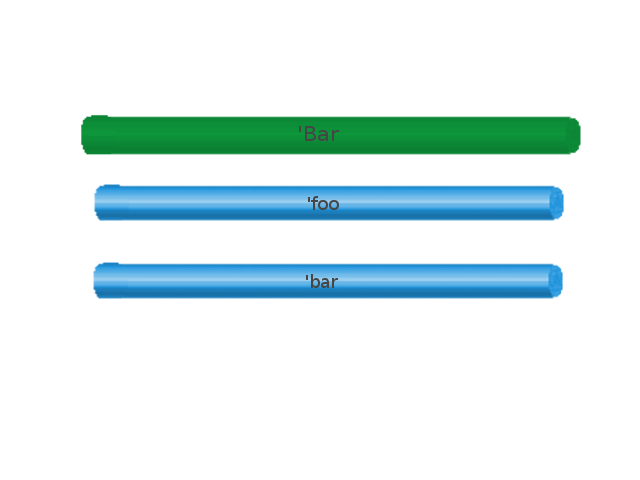
\includegraphics[width=5cm]{bar-owner}
    \end{column}
    \end{columns}
\end{frame}

\begin{frame}[fragile]
    \frametitle{Ownership}
    Entity vs Instance
    \begin{columns}[T]
    \begin{column}[T]{5.2cm}
    \begin{lstlisting}
    define a new entity {
        name = 'Bar
    }
    create a new instance {
        name = 'bar
    } of 'Bar
    define a new entity {
        name = 'Foo
        objects += (
            'bar
        )
    }
    \end{lstlisting}
    \end{column}

    \begin{column}[T]{5cm}
    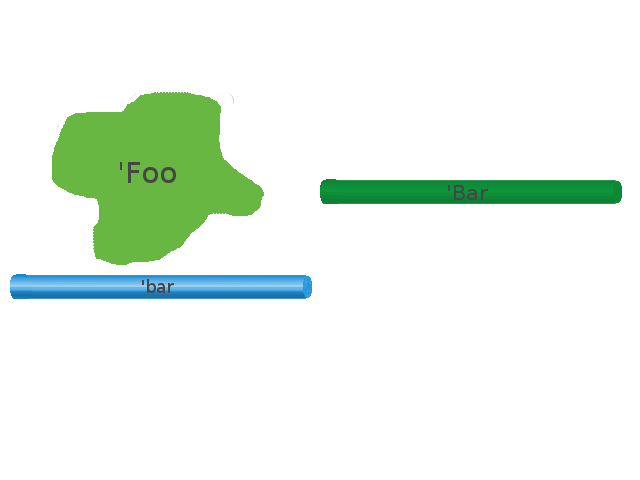
\includegraphics[width=5cm]{foo-bar-owner}
    \end{column}
    \end{columns}
\end{frame}

\begin{frame}[fragile]
    \frametitle{Ownership}
    \begin{lstlisting}
    nobody gives 'foo to 'bar
    // nobody gave 'foo to 'bar
    \end{lstlisting}
    \includegraphics<1>[width=13cm]{nobody-gives1}
    \includegraphics<2>[width=13cm]{nobody-gives2}
\end{frame}

\begin{frame}[fragile]
    \frametitle{Ownership}
    \begin{lstlisting}
    'bar gives 'foo to 'baz
    // 'bar gave 'foo to 'baz
    \end{lstlisting}
    \includegraphics<1>[width=13cm]{bar-gives1}
    \includegraphics<2>[width=13cm]{bar-gives2}
\end{frame}

\begin{frame}[fragile]
    \frametitle{Ownership}
    To check ownership:
    \begin{lstlisting}
    if('foo has 'bar)
    \end{lstlisting}

    To get a list of owned instances:
    \begin{lstlisting}
    'foo.inventory
    \end{lstlisting}
\end{frame}

\begin{frame}
    \frametitle{Actions}
    \begin{itemize}[<+->]
        \item{User-defined responses to actions}
        \item{Manual and automatic triggering}
        \item{Reusable}
    \end{itemize}
\end{frame}

\begin{frame}[fragile]
    \frametitle{Actions}
    \begin{lstlisting}
    define a new action {
        name = 'fooing
        action = (args: List[Any]) =>
            println("Fooooo!");
    }
    \end{lstlisting}
    
\includegraphics[width=10cm]{fooing}
\end{frame}

\begin{frame}[fragile]
    \frametitle{Actions}
    \begin{lstlisting}
    define a new action {
        name = 'fooing
        action = (args: List[Any]) =>
            println("Fooooo!");
        condition = () => amIReady()
    }
    \end{lstlisting}
    
\includegraphics[width=10cm]{fooing}
\end{frame}

\begin{frame}[fragile]
    \frametitle{Actions}
    \begin{columns}[T]
    \begin{column}[T]{5.5cm}
    \begin{lstlisting}
    define a new entity {
        name = 'Foo
        actions += (
            'fooing
        )
    }
    create a new instance {
        name = 'foo
    }
    \end{lstlisting}
    \end{column}
    \begin{column}[T]{4cm}
    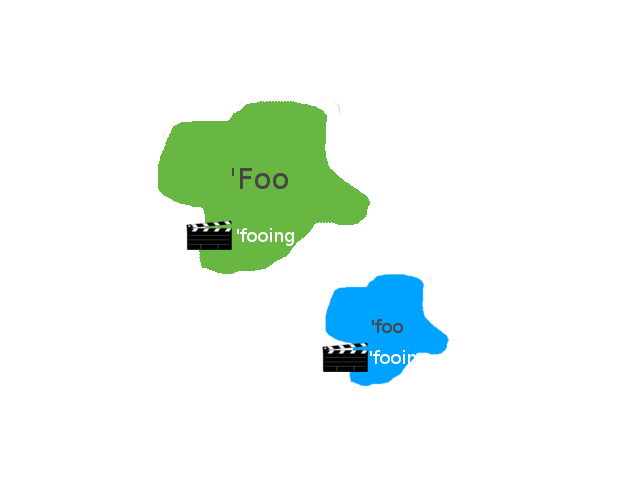
\includegraphics[scale=0.4, trim=8cm 0cm 8cm 0cm]{foo-fooing}
    \end{column}
    \end{columns}
\end{frame}

\begin{frame}[fragile]
    \frametitle{Actions}
    \begin{lstlisting}
    'foo does 'fooing using ()
    \end{lstlisting}
    \pause
    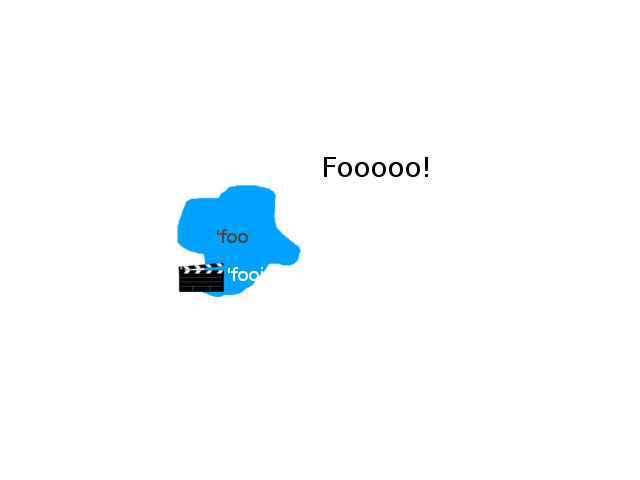
\includegraphics[width=13cm]{foo-inst-fooing}
\end{frame}

\begin{frame}[fragile]
    \frametitle{Actions}
    \begin{columns}[T]
    \begin{column}[T]{5cm}
    \begin{lstlisting}
    define a new entity {
        name = 'Foo
    }
    create a new instance {
        name = 'foo
        actions += (
            'fooing
        )
    } of 'Foo
    \end{lstlisting}
    \end{column}
    \begin{column}[T]{4cm}
    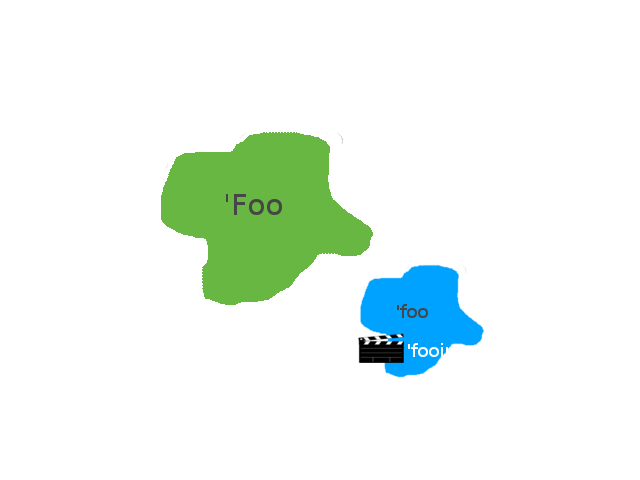
\includegraphics[scale=0.4, trim=8cm 0cm 8cm 0cm]{foo-Foo-fooing}
    \end{column}
    \end{columns}
\end{frame}

\begin{frame}[fragile]
    \frametitle{Actions}
    \begin{lstlisting}
    'foo does 'fooing using ()
    \end{lstlisting}
    \pause
    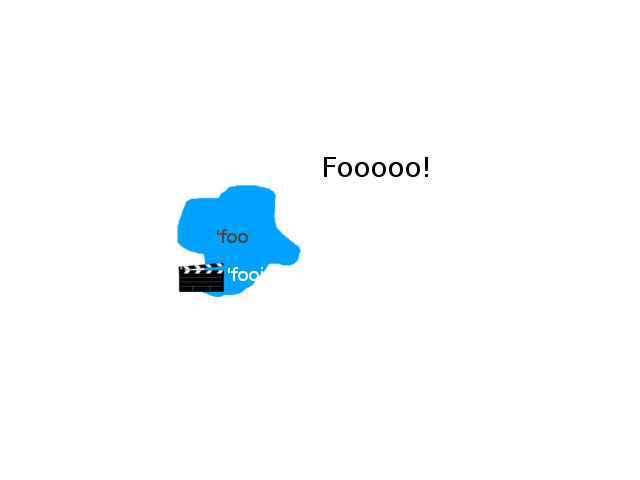
\includegraphics[width=13cm]{foo-inst-fooing}
\end{frame}

\begin{frame}
    \frametitle{Scenes}
    \begin{itemize}[<+->]
        \item{represent locations in the game}
        \item{can own Entities}
        \item{can have actions}
    \end{itemize}
\end{frame}

\begin{frame}[fragile]
    \frametitle{Scenes}
    \begin{lstlisting}
    create a new scene {
        name = 'Place1
        objects += (
            'foo,
            'baz
        )
        actions += (
            'fooing,
            'bazing
        )
    }
    nobody gives 'bar to 'Place1
    'Place1 gives 'bar to 'foo
    'foo gives 'bar to 'Place1
    'Place1 does 'bazing using (10, 11, 12)
    \end{lstlisting}
\end{frame}

{ %local backgrounds must be enclosed in braces
\usebackgroundtemplate{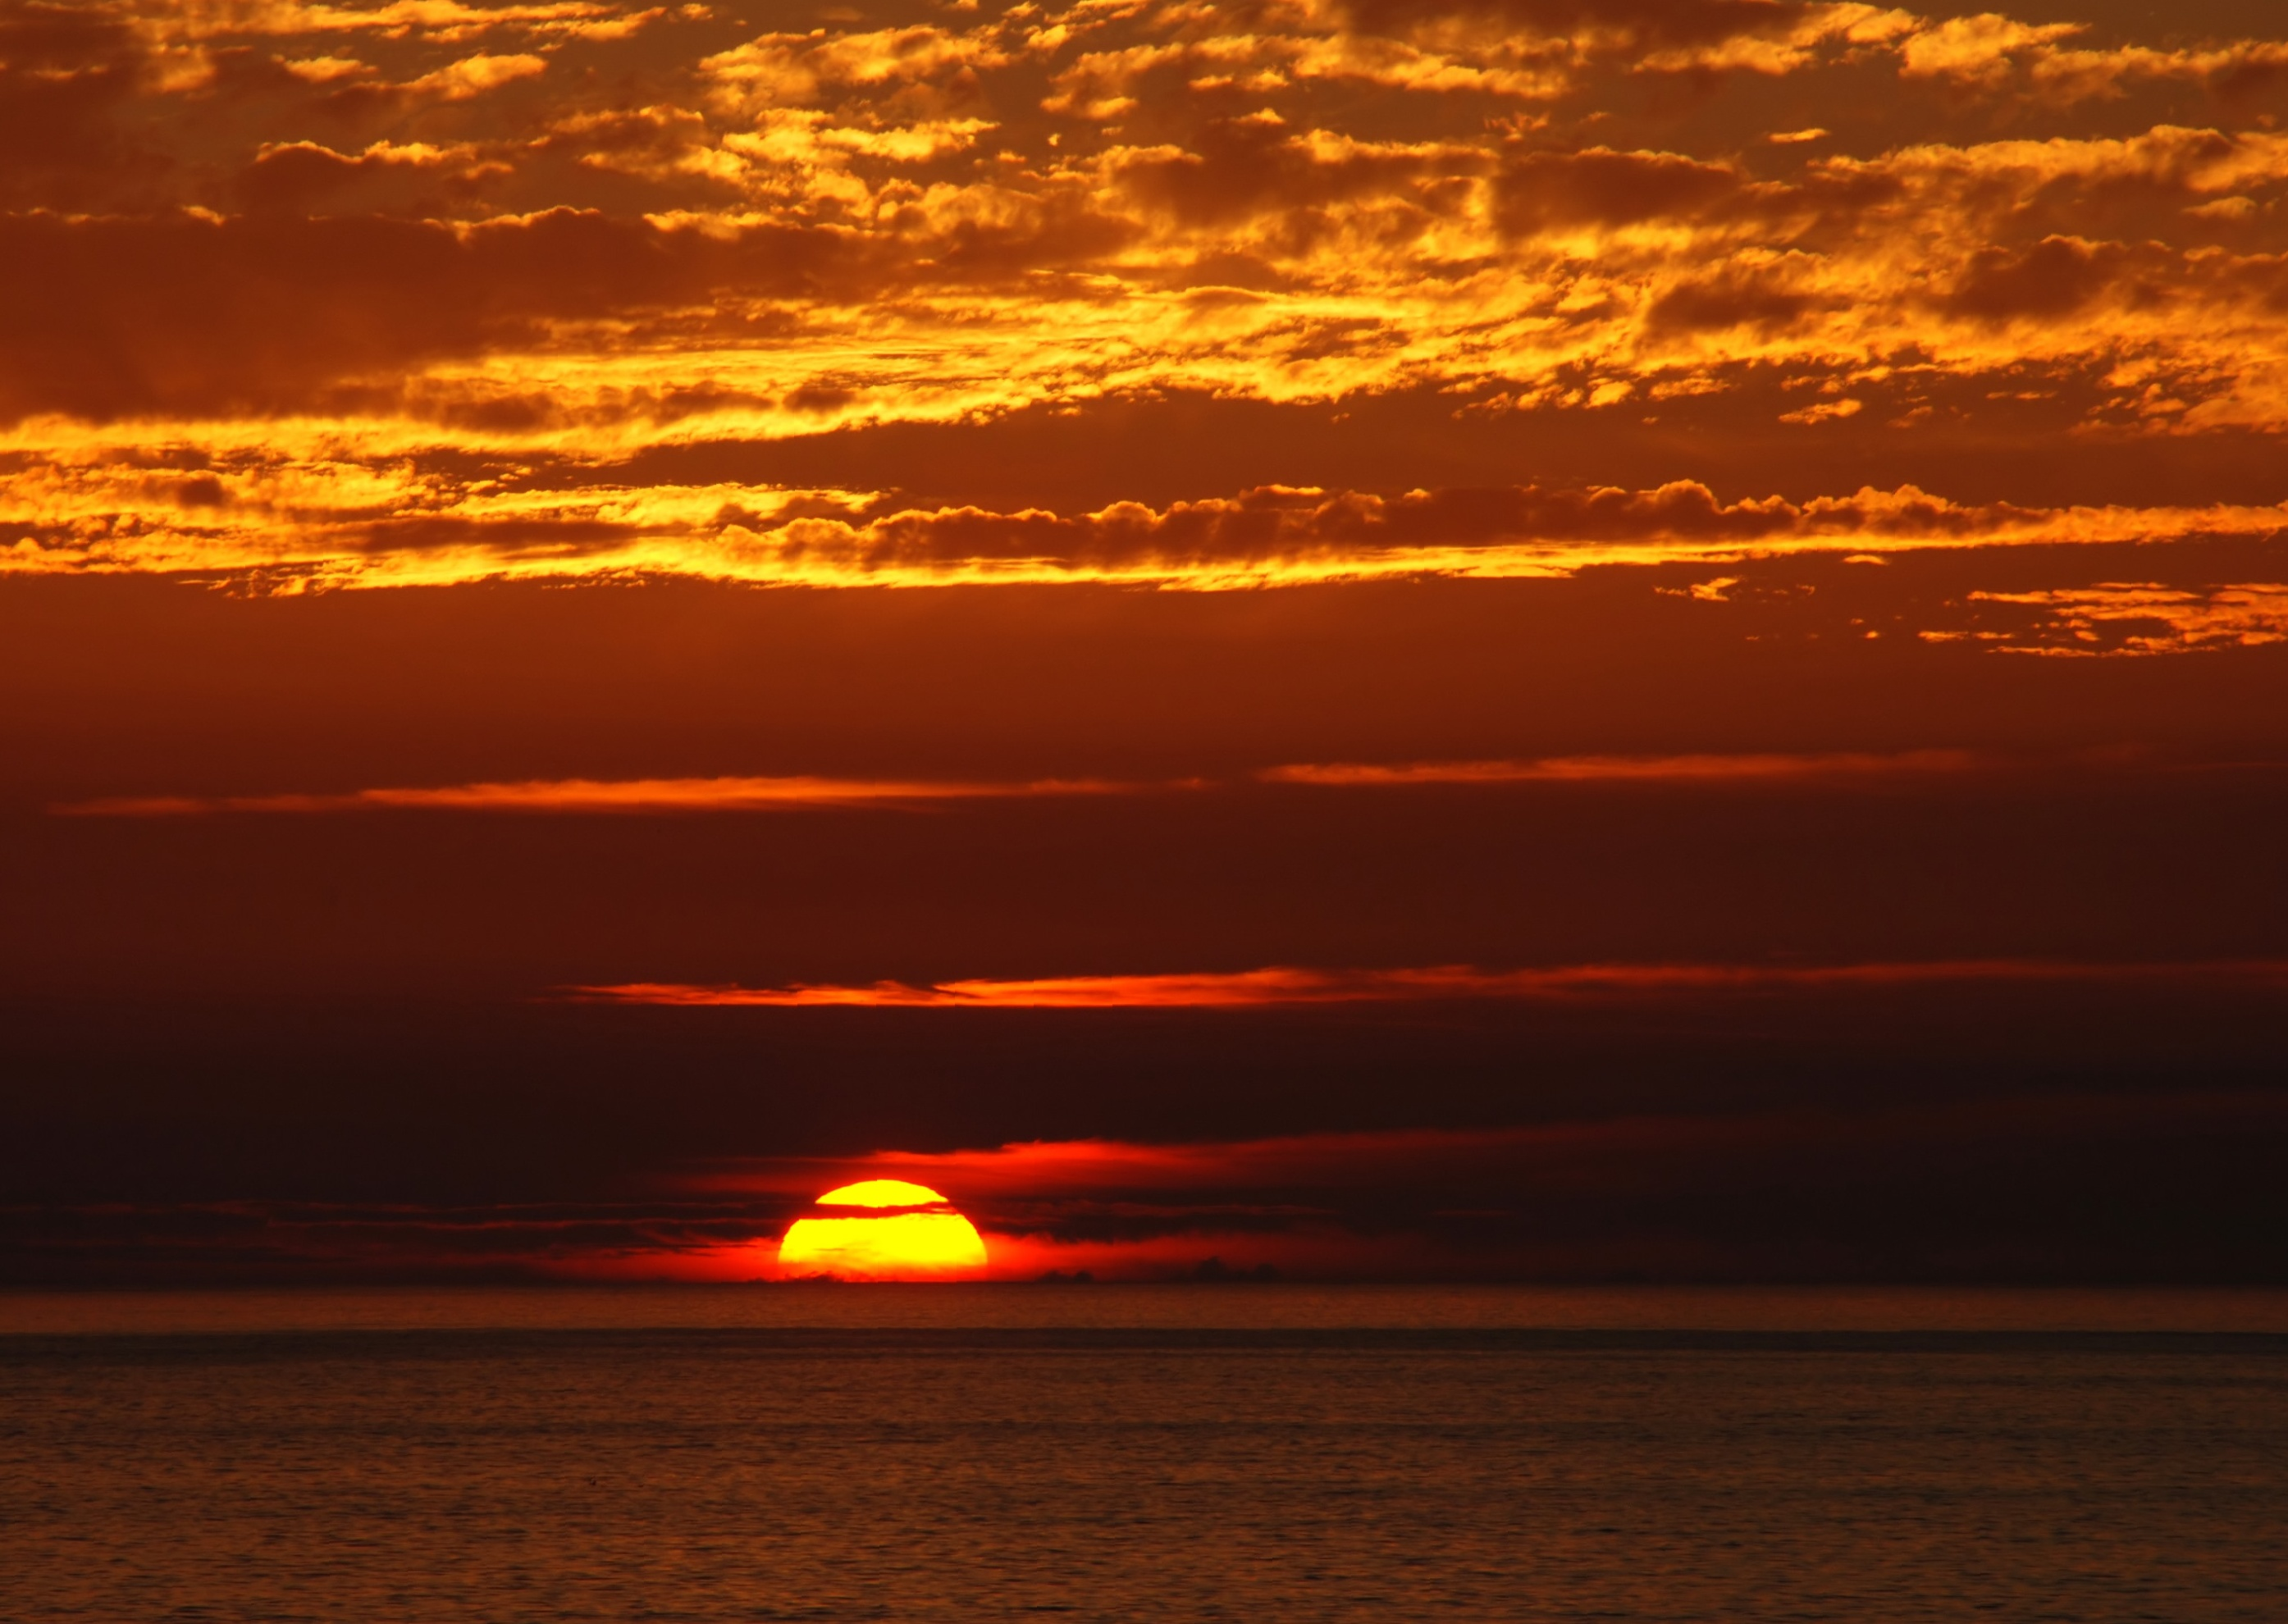
\includegraphics[width=\paperwidth]{scene.jpg}}

\begin{frame}
    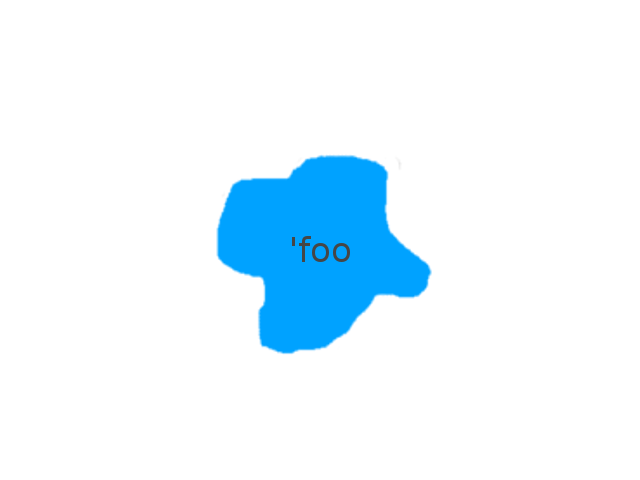
\includegraphics[width=4cm, trim= 4cm 4cm 4cm 4cm]{foo-instance}
    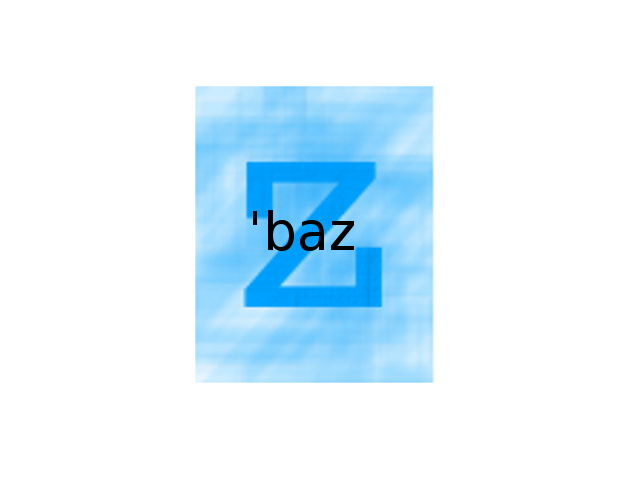
\includegraphics[width=4cm, trim= 4cm 4cm 4cm 4cm]{baz-instance}
    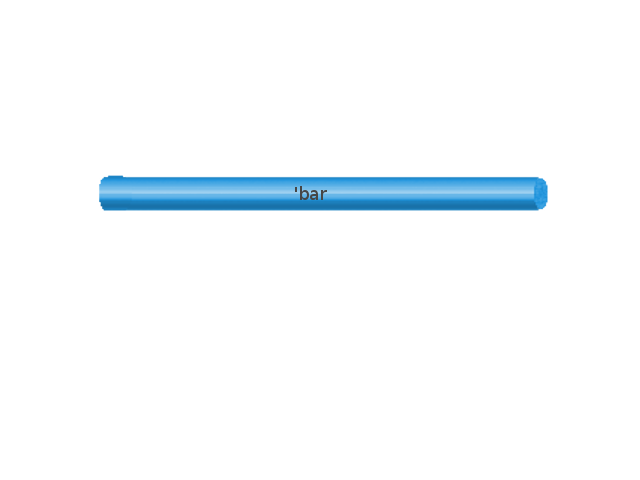
\includegraphics[width=4cm, trim= 4cm 4cm 4cm 4cm]{bar-instance}
\end{frame}

\begin{frame}
    \begin{columns}[T]
    \begin{column}[T]{5cm}
    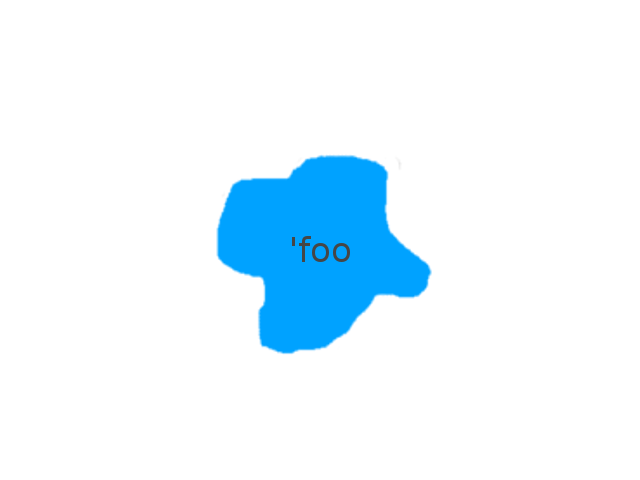
\includegraphics[width=5cm, trim= 4cm 4cm 4cm 4cm]{foo-instance}\\
    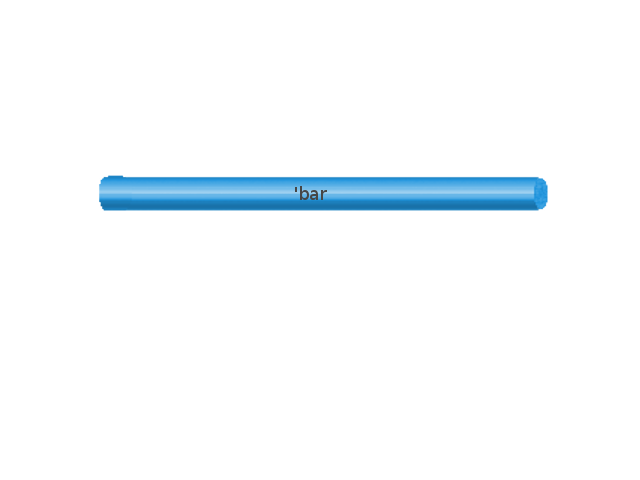
\includegraphics[width=5cm, trim= 4cm 4cm 4cm 4cm]{bar-instance}
    \end{column}
    \begin{column}[T]{4cm}
    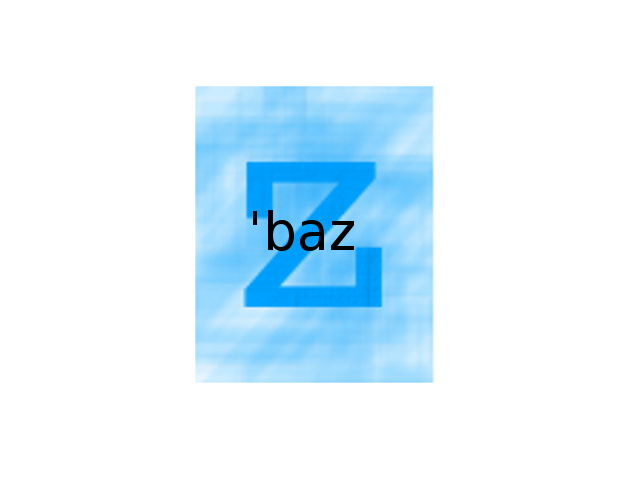
\includegraphics[width=5cm]{baz-instance}
    \end{column}
    \end{columns}
\end{frame}

\begin{frame}
    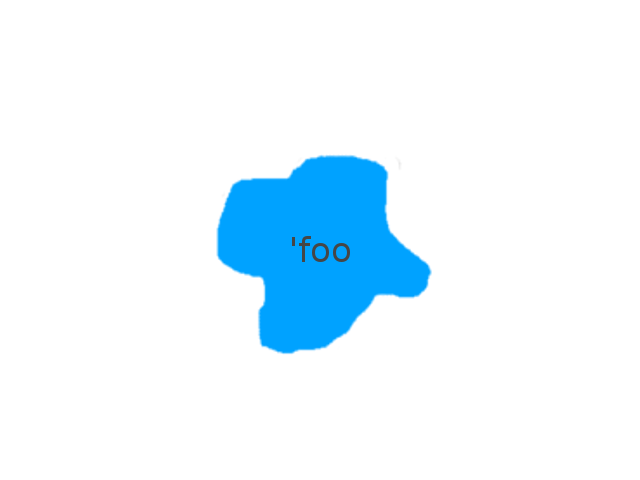
\includegraphics[width=4cm, trim= 4cm 4cm 4cm 4cm]{foo-instance}
    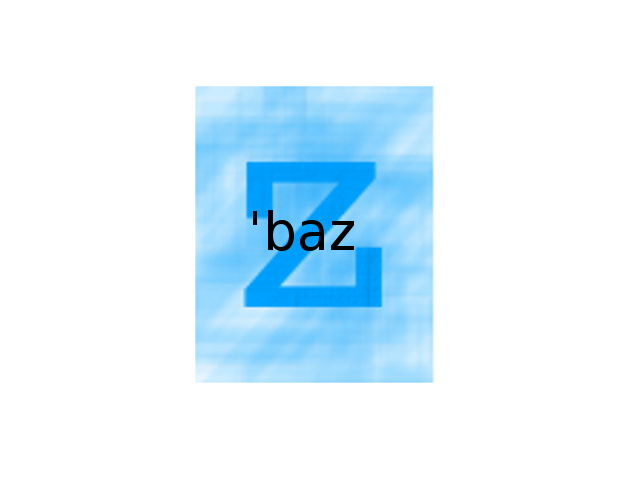
\includegraphics[width=4cm, trim= 4cm 4cm 4cm 4cm]{baz-instance}
    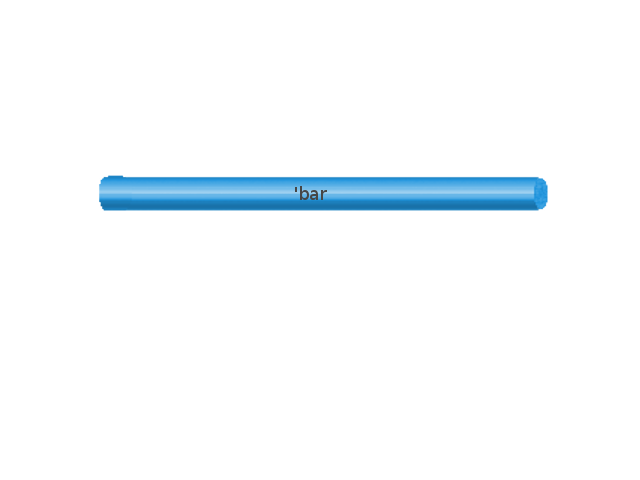
\includegraphics[width=4cm, trim= 4cm 4cm 4cm 4cm]{bar-instance}

    \pause

    \begin{center}
    \color{green}
    \huge{Bazzzz!!}
    \end{center}
\end{frame}
}

\begin{frame}[fragile]
    \frametitle{Game}
    The game object contains the settings of the game
    \begin{lstlisting}
    create a new game {
        name = "Hello World! Adventure"
        description = "Hello World!"
        resolution = (1024, 512)
        startScene = 'StartScene
        fps = 60 // optional, default=30
    }
    \end{lstlisting}
\end{frame}

\begin{frame}
    \frametitle{Graphics}
    \begin{itemize}[<+->]
        \item{Integrated with Swing}
        \item{Automatic rendering}
        \item{Support for backgrounds}
    \end{itemize}
\end{frame}

\begin{frame}
    \frametitle{Graphics}
    \framesubtitle{GamelRenderer}
    \begin{itemize}[<+->]
        \item{Encapsulates rendering info and methods}
        \item{Can use with scenes or entities}
    \end{itemize}
\end{frame}

\begin{frame}[fragile]
    \frametitle{Graphics}
    \framesubtitle{GamelRenderer}
    Just subclass GamelRenderer:
    \begin{lstlisting}[basicstyle=\small]
    object SceneRenderer extends GamelRenderer {
        def render(self: GamelEntity,
                    g2d: Graphics2D): Unit = <function>
    }
    \end{lstlisting}
\end{frame}

\begin{frame}[fragile]
    \frametitle{Graphics}
    \framesubtitle{GamelRenderer}
    Pass the GamelRenderer to the scene, entity, or instance:
    \begin{lstlisting}[basicstyle=\small]
    define a new entity {
        name = 'Foo
        renderer = FooRenderer
    }
    \end{lstlisting}
    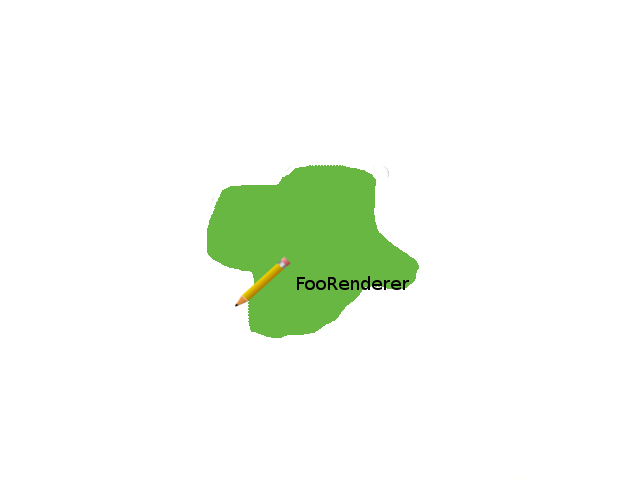
\includegraphics[width=10cm, trim= 4cm 4cm 4cm 4cm]{Foo-render}
\end{frame}
\begin{frame}[fragile]
    \frametitle{Graphics}
    \framesubtitle{GamelRenderer}
    Pass the GamelRenderer to the scene, entity, or instance:
    \begin{lstlisting}[basicstyle=\small]
    create a new instance {
        name = 'bar
        renderer = BarRenderer
    } of 'Bar
    \end{lstlisting}
    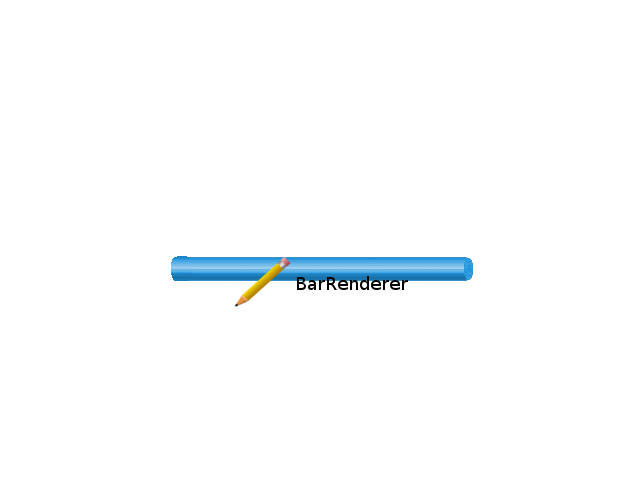
\includegraphics[width=10cm, trim= 4cm 4cm 4cm 4cm]{bar-render}
\end{frame}

\begin{frame}[fragile]
    \frametitle{Graphics}
    \framesubtitle{GamelRenderer}
    Pass the GamelRenderer to the scene, entity, or instance:
    \begin{lstlisting}[basicstyle=\small]
    create a new scene {
        name = 'Sunset
        renderer = SceneRenderer
    }
    \end{lstlisting}
    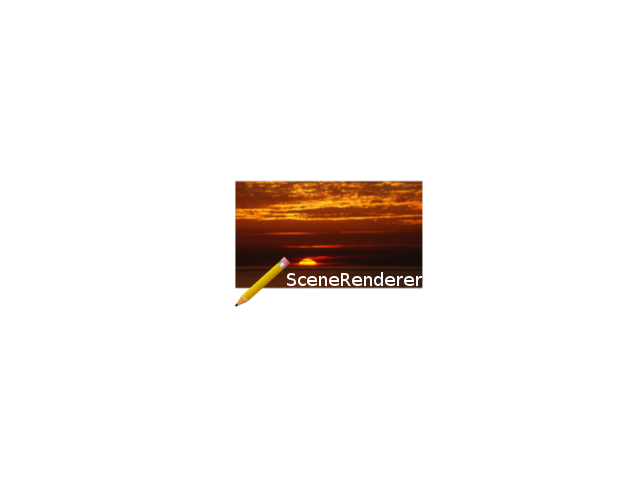
\includegraphics[width=10cm, trim= 4cm 4cm 4cm 4cm]{scene-render}
\end{frame}

\begin{frame}
    \frametitle{Graphics}
    \framesubtitle{Rendering}
    \begin{itemize}[<+->]
        \item{All of the current scene's objects are rendered}
        \item{If an entity is rendered, all of its objects are too}
        \item{If an entity or scene does not have a renderer, it is not rendered}
    \end{itemize}
\end{frame}

\begin{frame}[fragile]
    \frametitle{Graphics}
    \framesubtitle{Switching scenes}
    \begin{lstlisting}
    go to 'Moonrise
    \end{lstlisting}
    \includegraphics<1>[width=5cm]{scene}
    \includegraphics<2>[width=5cm]{transition}
\end{frame}

\begin{frame}
    \frametitle{Graphics}
    \framesubtitle{Require and Use}
    \begin{itemize}[<+->]
        \item{Support for more easily using images in game design}
        \item{Allows "aliasing" of images}
        \item{The GamelRenderer also has a \texttt{scene} field for backgrounds}
    \end{itemize}
\end{frame}

\begin{frame}[fragile]
    \frametitle{Graphics}
    \framesubtitle{Require and Use}
    \begin{lstlisting}
     require image "sunset.jpg" as "bg"
     // now sunset.jpg can be refered to as "bg"

     ...

     object SceneRenderer extends GamelRenderer {
        var scene = use image "bg"
        // using image as the bg
        def render...
     }
    \end{lstlisting}
\end{frame}

\begin{frame}
    \frametitle{Event handling}
    Support for many keyboard and mouse events:
    \begin{multicols}{2}
    \begin{itemize}[<+->]
        \item{Key press and release}
        \item{Typing}
        \item{Clicking}
        \item{Mouse over}
        \item{Mouse moving}
        \item{Mouse press and release}
        \item{Dragging}
        \item{Scrolling}
    \end{itemize}
    \end{multicols}
\end{frame}

\begin{frame}[fragile]
    \frametitle{Event handling}
    To toggle an event handler:
    \begin{columns}[T]
    \begin{column}[T]{5cm}
    \begin{lstlisting}
    turn KeyPress on
    turn MousePress off
    ...
    \end{lstlisting}

    To detect an event:
    \begin{lstlisting}
    detect KeyPress
    \end{lstlisting}
    \end{column}
    \begin{column}[T]{5cm}
    
\includegraphics[width=5cm]{keyboard}
    \end{column}
    \end{columns}
\end{frame}

\begin{frame}[fragile]
    \frametitle{Starting the game}
    \begin{center}
        \huge{
            \texttt{start game}
        }
    \end{center}
\end{frame}

\begin{frame}
    \frametitle{Advantages of GameL}
    \begin{itemize}[<+->]
        \item{Modular}
        \item{Easy to learn}
        \item{Easy to read}
        \item{Easy to use}
        \item{Lazy evaluation => no forward declaration}
        \item{Flexible}
    \end{itemize}
\end{frame}

\begin{frame}[plain,c]
    \begin{center}
        \Huge DEMO
    \end{center}
\end{frame}

\end{document}
